%   ------------------------------------------------------------------------
\FloatBarrier
\section{Análise do SpriteSheetGPT}
\label{s.spriteSheetGPT}

A ferramenta SpriteSheetGPT, encontrada no site YesChat.AI, à primeira vista parecia promissora por seu aparente foco na criação de sprite sheets, como seu nome sugere. O objetivo principal do teste era produzir o sprite sheet do walking cycle do personagem utilizando o sprite de Pablo em front view (Figura \ref{fig:Pablo}). 

Contudo, em experimentos iniciais realizados durante junho, ao receber o prompt, a ferramenta demonstrou um comportamento curioso. Conforme é mostrado na Figura \ref{fig:yesAI1Edit}, ao receber o prompt a IA solicita o reenvio da imagem de referência e, em uma tentativa subsequente, descreveu textualmente o sprite sheet a ser gerado. Somando a todos esses fatores, a ferramenta também tem um uso gratuito limitado, requerendo uma inscrição paga para continuar a ser usada em um período de tempo incerto, conforme demonstrado na Figura \ref{fig:yesAILimitado} do Apêndice \ref{ap.telasIA}. Com base nesse comportamento, a ferramenta inicialmente foi descartada. A captura de tela completa desta interação pode ser consultada na Figura \ref{fig:yesAI1} do Apêndice \ref{ap.telasIA}.


\begin{figure}[htbp]
    \centering
    \caption{\small Tela do SpriteSheetGPT não gerando o resultado esperado}
    \label{fig:yesAI1Edit}

    \begin{subfigure}{1\linewidth}
        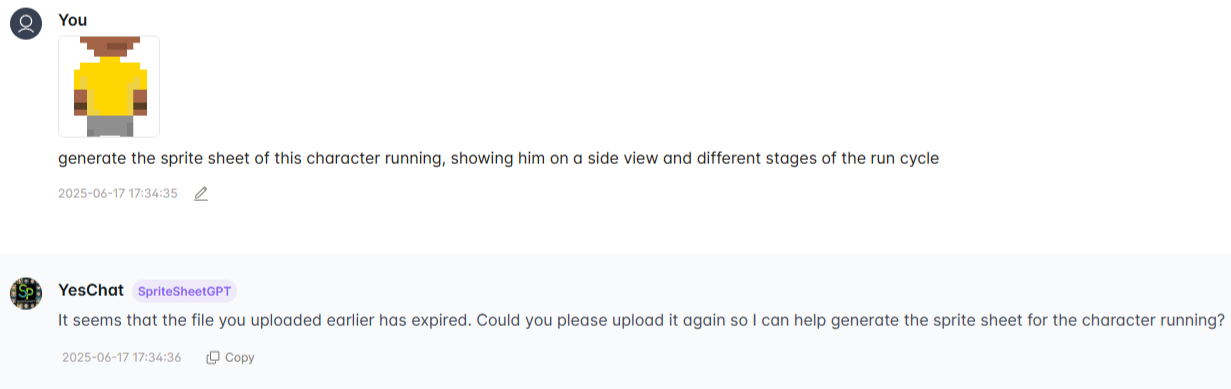
\includegraphics[width=1\linewidth]{figs/yesAI/mono1.PNG}
        \caption{\small Comportamento inesperado ao pedir reenvio da imagem}
        \label{fig:yesAI1aEdit}
    \end{subfigure}
    \begin{subfigure}{1\linewidth}
        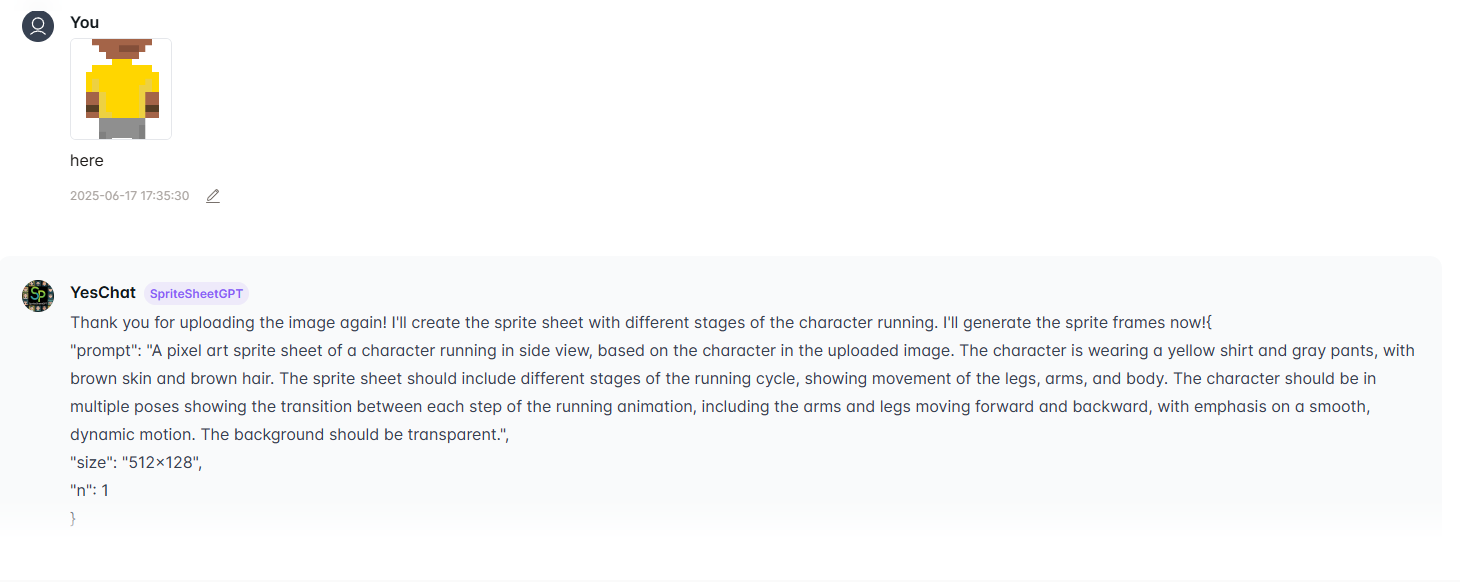
\includegraphics[width=1\linewidth]{figs/yesAI/tela2.PNG}
        \caption{\small Descrição textual do sprite sheet em vez de gerar a imagem.}
        \label{fig:yesAI1bEdit}
    \end{subfigure}

    \legend{\small Fonte: Elaborada pela autora.}
\end{figure}

Com o decorrer das semanas, a ferramenta foi testada mais algumas vezes sem nenhum resultado distinto do já apresentado. Devido ao comportamento se manter o mesmo, não foi registrada nenhuma nova captura de tela.

%sim, 24 de agosto foi quando eu estava escrevendo

No entanto, em uma nova verificação realizada em 24 de agosto de 2025, a IA apresentou uma resposta diferente das anteriores. Após a resposta textual inicial, ela procedeu para a geração da imagem. O artefato resultante (Figura \ref{fig:yesAIResultado}) demonstrou baixa consistência com a imagem de referência, tendo cores apenas vagamente semelhantes; apresentou baixa precisão com o prompt, sem representar o personagem andando; e reproduziu apenas parcialmente o estilo de pixel art. O único ponto positivo é que foi formado um sprite sheet de um personagem em 2D. A interação completa pode ser vista na Figura \ref{fig:yesAI2} do Apêndice \ref{ap.telasIA}

\begin{figure}[htbp]
    \centering
    \caption{\small Sprite sheet gerado pelo SpriteSheetGPT}
    \label{fig:yesAIResultado}
    
\includegraphics[width=1\linewidth]{figs/yesAI/resultado.png}
    \legend{\small Fonte: Elaborada pela autora, utilizando a ferramenta SpriteSheetGPT.}
\end{figure}

Ao tentar replicar a geração com os mesmos prompt e imagem de referência, novamente a ferramenta voltou a apenas gerar um resultado textual (Figura \ref{fig:yesAI3} do Apêndice \ref{ap.telasIA}).

Portanto, mesmo após conseguir produzir uma imagem, a conclusão da análise é que a ferramenta se mostra extremamente instável para qualquer aplicação prática no momento. A incapacidade de reproduzir um resultado preciso em relação ao prompt e consistente com a imagem de referência, além da ocasional falta de resultado visual, são falhas críticas. 

Apesar do descarte da ferramenta, seu comportamento destaca um aspecto fundamental dos modelos de IA generativa: a variabilidade de resultados para um mesmo input. Essa aleatoriedade (controlada pela seed de geração) demonstra a importância de que o usuário realize múltiplas iterações da mesma instrução para alcançar um resultado satisfatório. Em modelos com uso gratuito limitado, essa necessidade de re-geração torna o sucesso dependente da sorte, uma vez que o resultado desejado pode não ser alcançado dentro do limite de tentativas disponíveis.